\section{Systematic uncertainties}
\label{sec:syst}

\todo{fix citations}
\subsection{Theory uncertainties}
\label{ssec:theoryuncert}

The estimation of the CP BSM parameters, $\tilde{d}$\todo{mention explicitly}, from the OO shape requires the precise knowledge of the SM contributions and related uncertainties. This includes both SM gluon-gluon fusion (background) and SM VBF (signal).
 Therefore, the different theoretical uncertainties affecting the SM predictions are included in the fitting likelihood. This includes uncertainties arising from the imperfect knowledge of:
 \begin{itemize}
 	\item missing higher-order terms in the perturbative QCD calculations;
 	\item the parton density functions (PDF) and the value of the strong coupling constant, $\alpha_{s}$;
 	\item the QCD effects in the soft and collinear regime, hadronization and multi-parton interactions;
 \end{itemize}

For the gluon-fusion production mode, nine uncertainty sources are used to model the QCD theory
uncertainties, following the recommendation of the LHC Higgs cross section working group~\cite{LHCXS_4}. These sources are:
\begin{itemize}
\item two sources correspond to yield uncertainties related to the total cross section. Their magnitude is taken from the
STWZ-BLPTW predictions~\cite{ggF_qcd_unc_1,ggF_qcd_unc_2,LHCXS_4} and their impact on the different bins is evaluated using
NNLOPS.
\item two sources correspond to migration uncertainties related to splitting the phase space by jet multiplicity. Their magnitude and impact are derived similarly to the yield uncertainties
\item two uncertainty sources are related to the $p_\mathrm{T}^H$ shape and are estimated from scale
variations in NNLOPS, including variations of the HNNLO input scales and the renormalization
and factorization scales in Powheg.
\item two uncertainty sources related to the enhancement of uncertainties for events with typical VBF topology (due to explicit or implicit third-jet vetos), and are estimated by scale variations in MCFM~\cite{MCFM}, and the corresponding uncertainties are estimated using the same procedure use for yield and migration uncertainties.
\item one uncertainty source is related to the treatment of $m_t$ and is most important at large $p_\mathrm{T}^H$.
\end{itemize}

For the \textcolor{red}{why VH}$VBF+VH$ production modes, QCD uncertainties are estimated as an envelope of the scale variations available in Powheg~\cite{Nason:2009ai,VBFVH_theoryUnc}. Uncertainties from the choice of the PDF set and $\alpha_\mathrm{s}$ are evaluated similar to the gluon-fusion case.

Following the recommendations of PDF4LHC~\cite{pdf4lhc}, the PDF uncertainties are evaluated using the 30 eigenvectors\todo{eigenvariations} set and treating each of them as an uncorrelated source. One additional nuisance parameter accounts for the uncertainties in $\alpha_{s}$.

\textcolor{red}{need plots} Parton shower systematics are estimated by varying the nominal parton shower algorithm Pythia with the alternative Herwig. These are therefore 2 uncorrelated NPs uncertainties and are computed for each category and for each truth bin.

A summary of the magnitude of these uncertainties in the different categories and OO bins is shown in the Figure ~\ref{fig:theoryUnc_ggF} ~\ref{fig:theoryUnc_VBF}. Roughly, among all the 4 categories, the QCD, PDF, $\alpha_{s}$ and total theory uncertaities are 10\textasciitilde22\% (2\textasciitilde5\%), 1.5\textasciitilde2.5\% (1\textasciitilde2\%), 4\textasciitilde5\% (\textasciitilde1\%) and 10\textasciitilde23\% (2\textasciitilde5\%) for ggF (VBF).
\todo{add a comment on the rough size of these uncertainties}
\todo{plots are too small}
\begin{figure}[htbp]
\centering
  \subfloat[TT ]{ 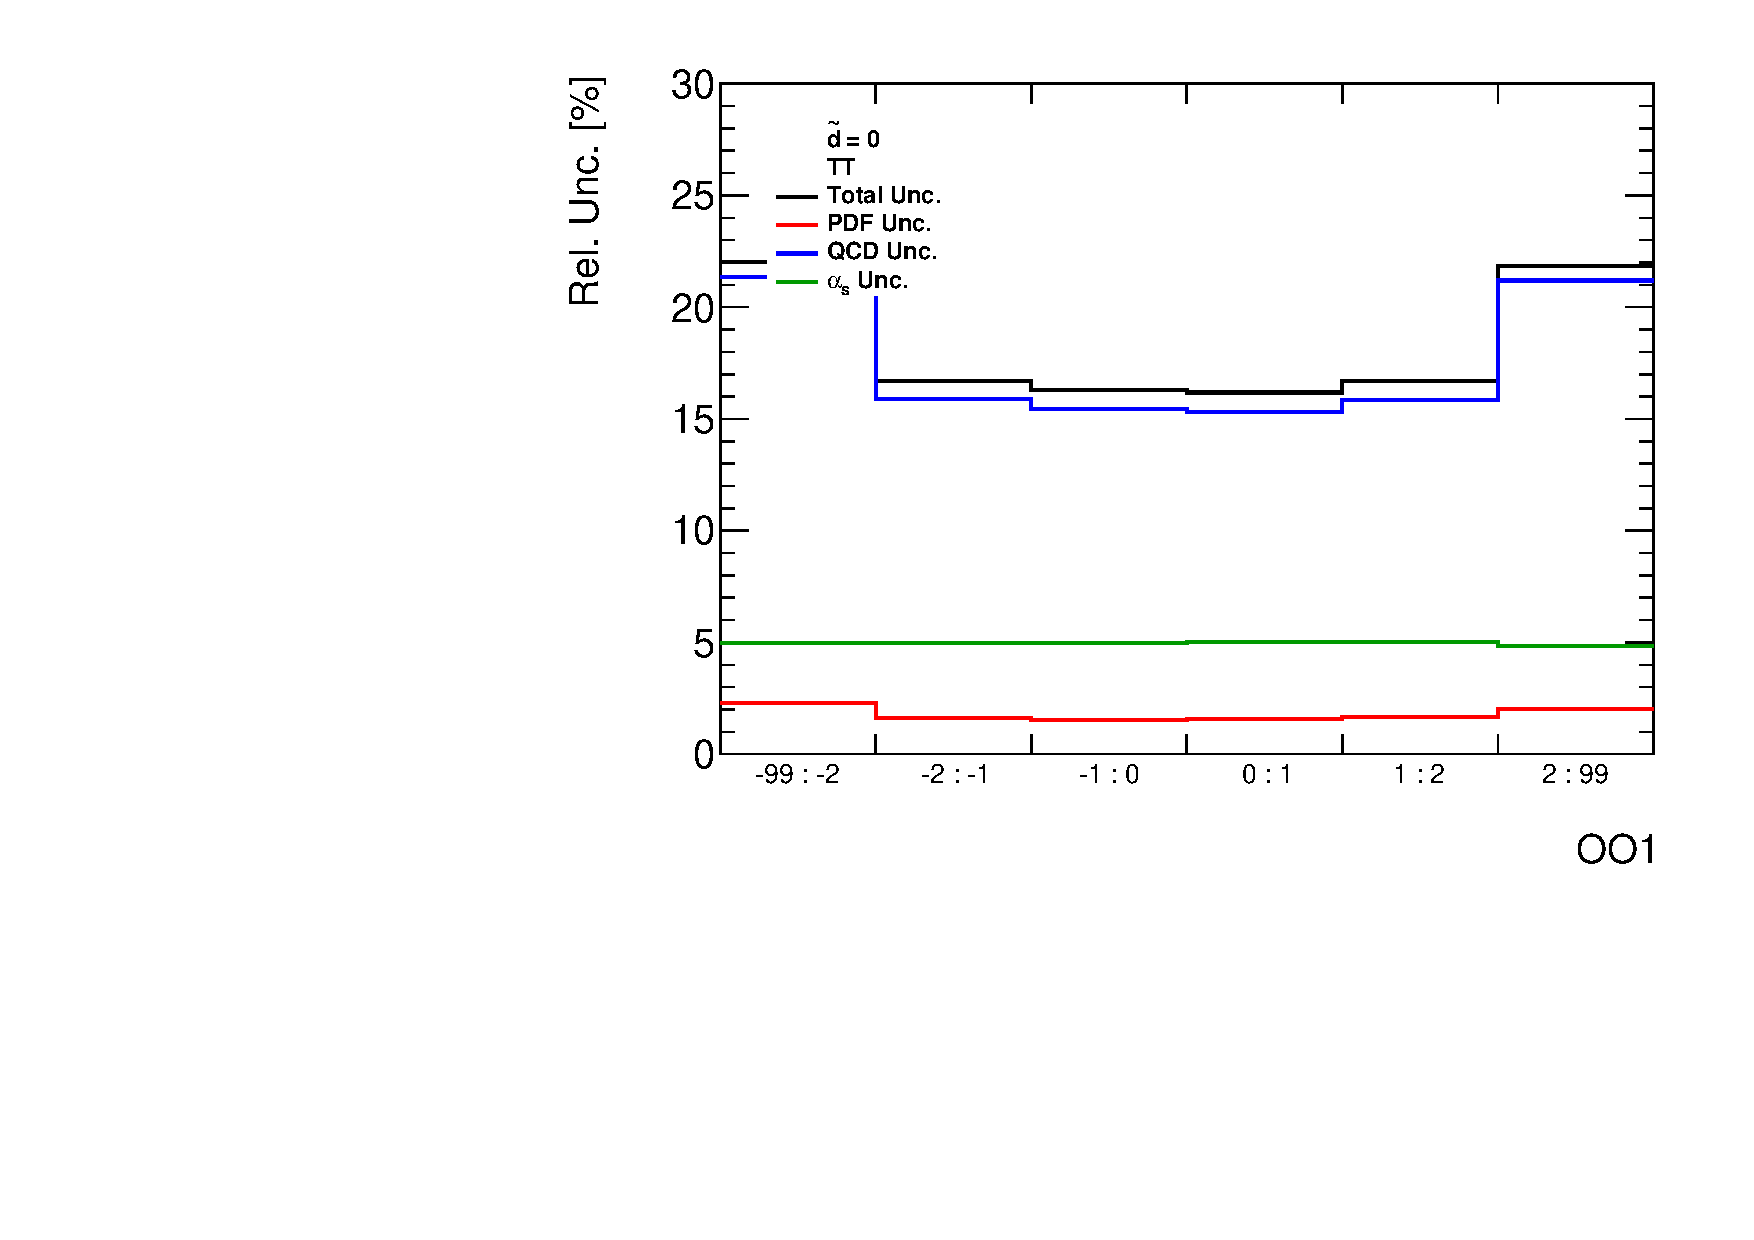
\includegraphics[width= 0.5\textwidth]{figure/TheorySyst/ggF_theoryUnc_TT_d_0.pdf} }
  \subfloat[TL ]{ 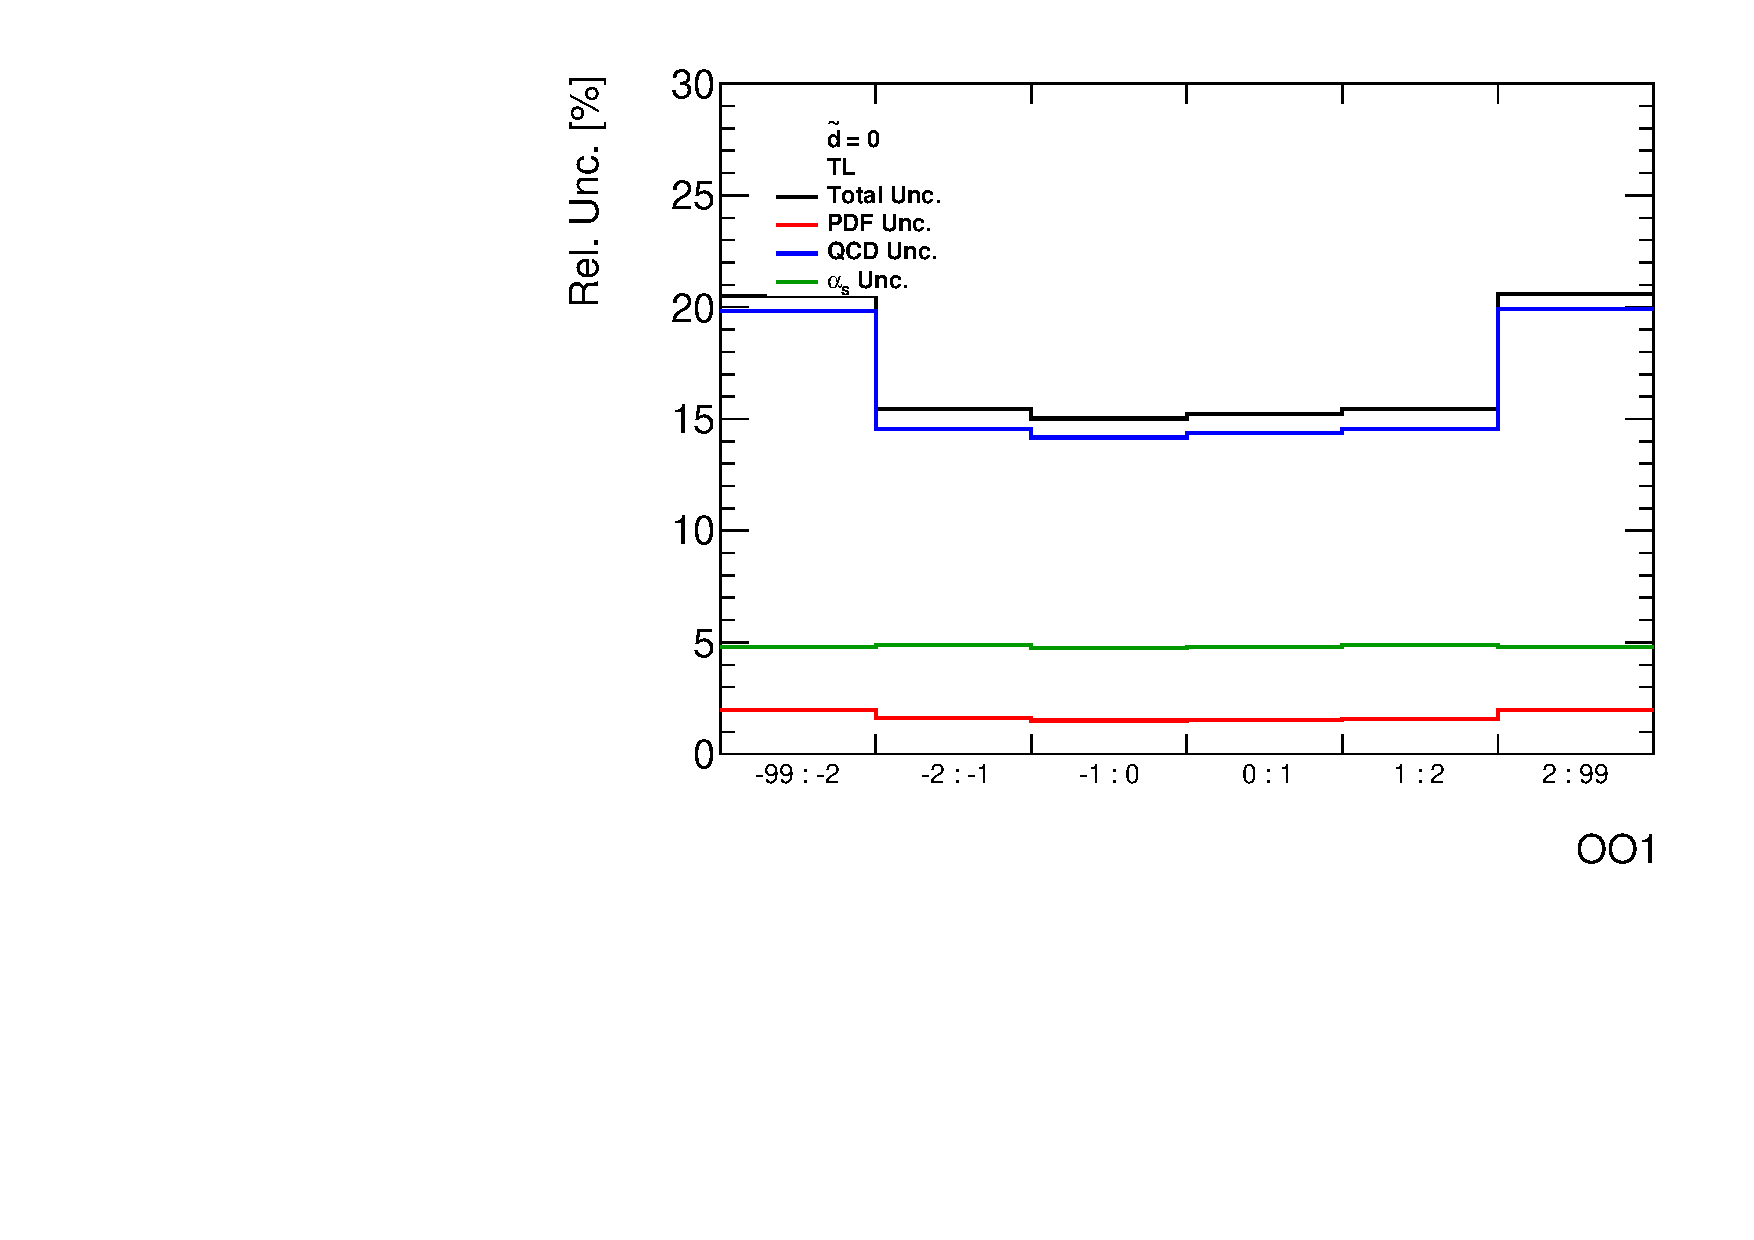
\includegraphics[width= 0.5\textwidth]{figure/TheorySyst/ggF_theoryUnc_TL_d_0.pdf} }\\
  \subfloat[LT ]{ 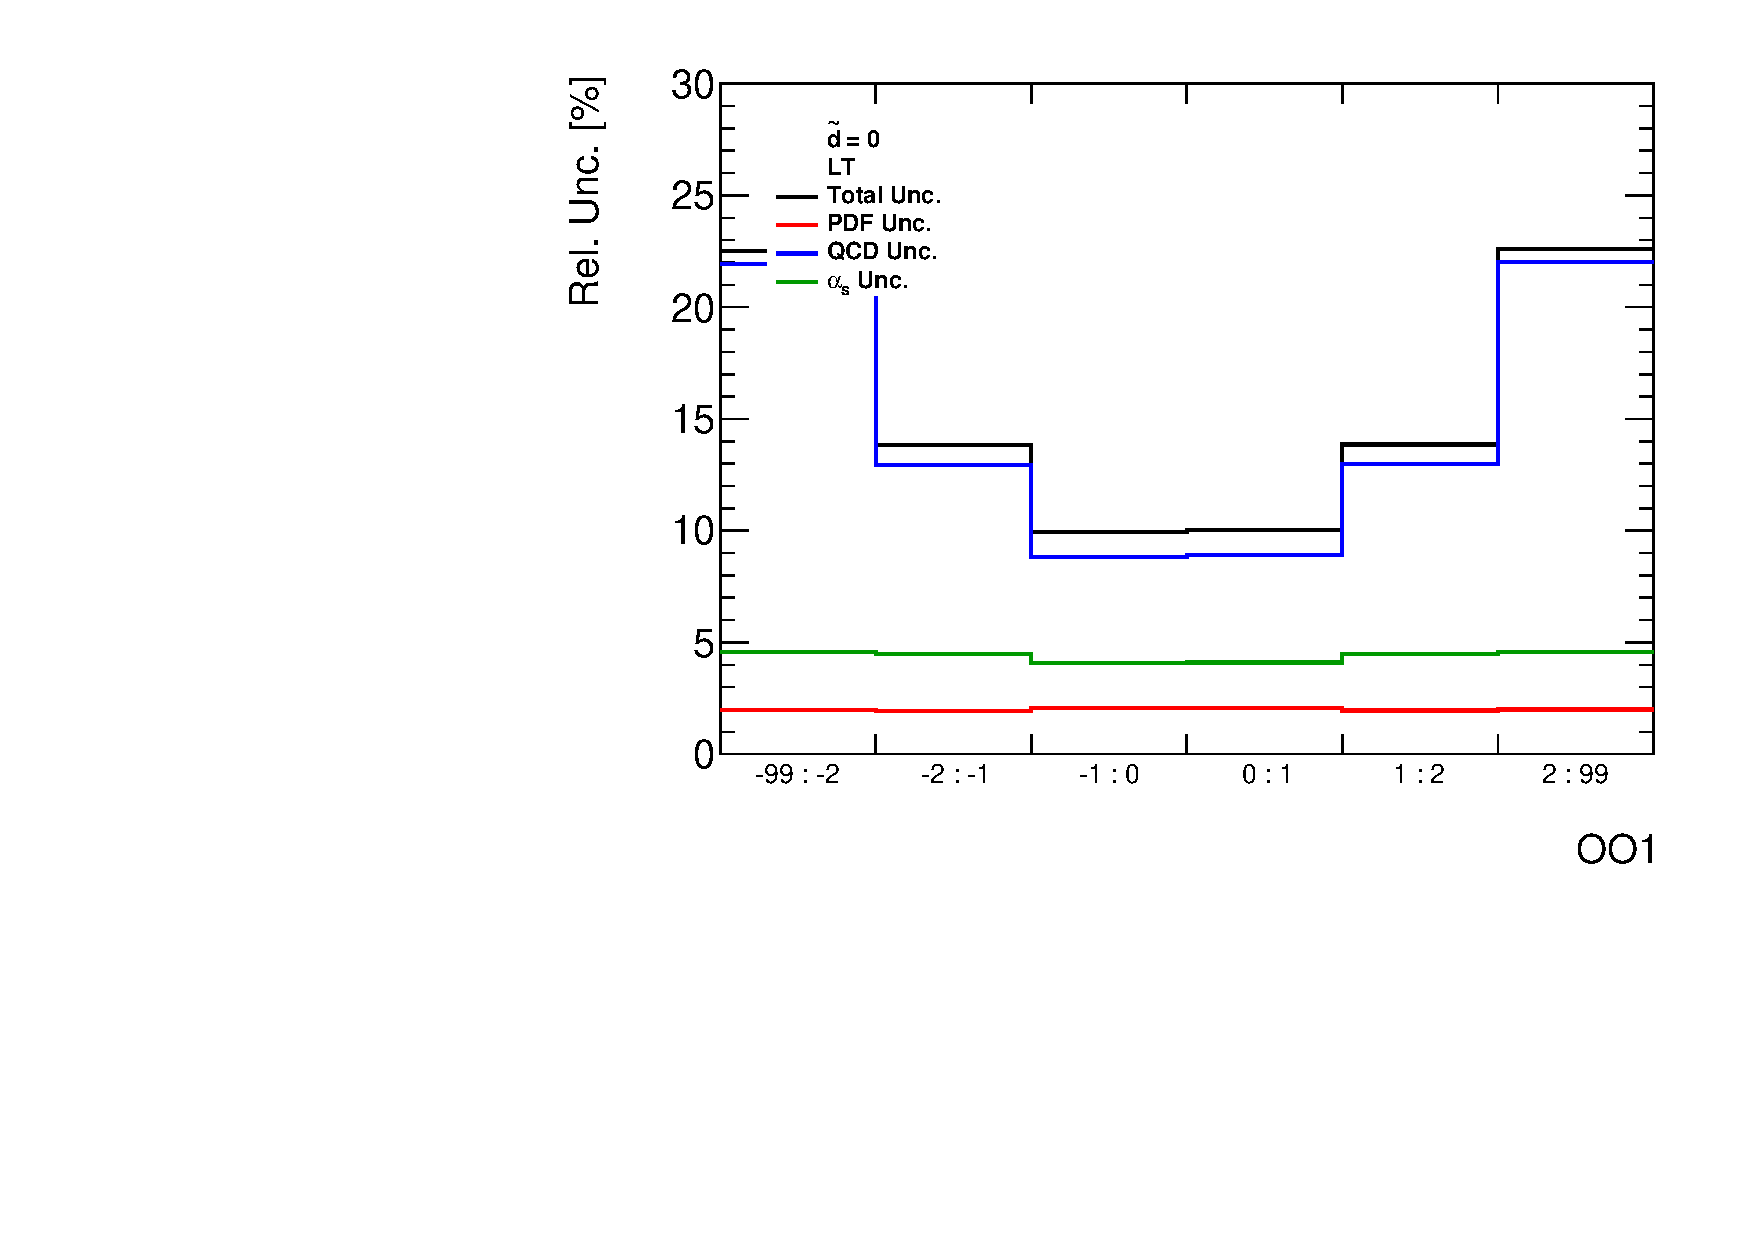
\includegraphics[width= 0.5\textwidth]{figure/TheorySyst/ggF_theoryUnc_LT_d_0.pdf} } 
  \subfloat[LL ]{ 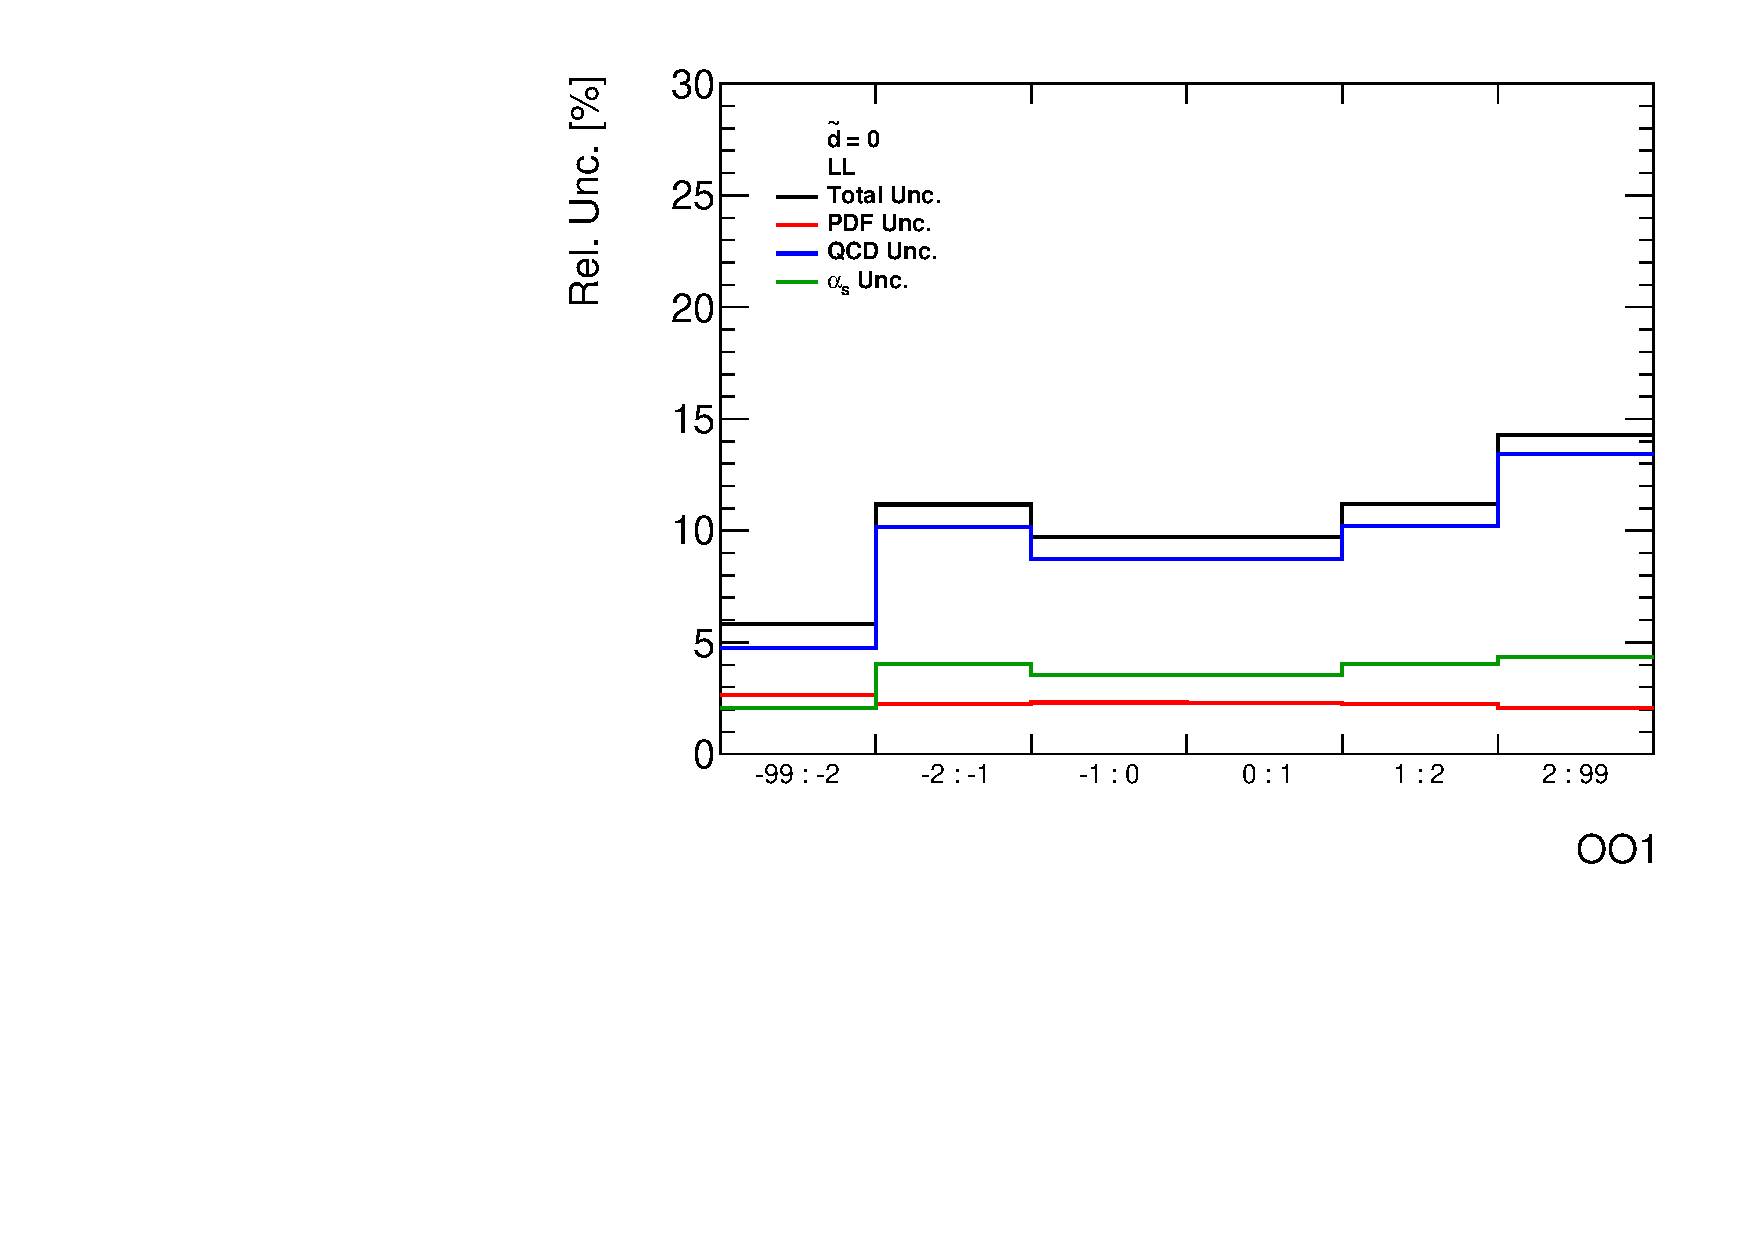
\includegraphics[width= 0.5\textwidth]{figure/TheorySyst/ggF_theoryUnc_LL_d_0.pdf} } 
  \caption{Theory uncertainty in different OO bins for ggF process}
  \label{fig:theoryUnc_ggF}
\end{figure}

\begin{figure}[htbp]
\centering
  \subfloat[TT ]{ 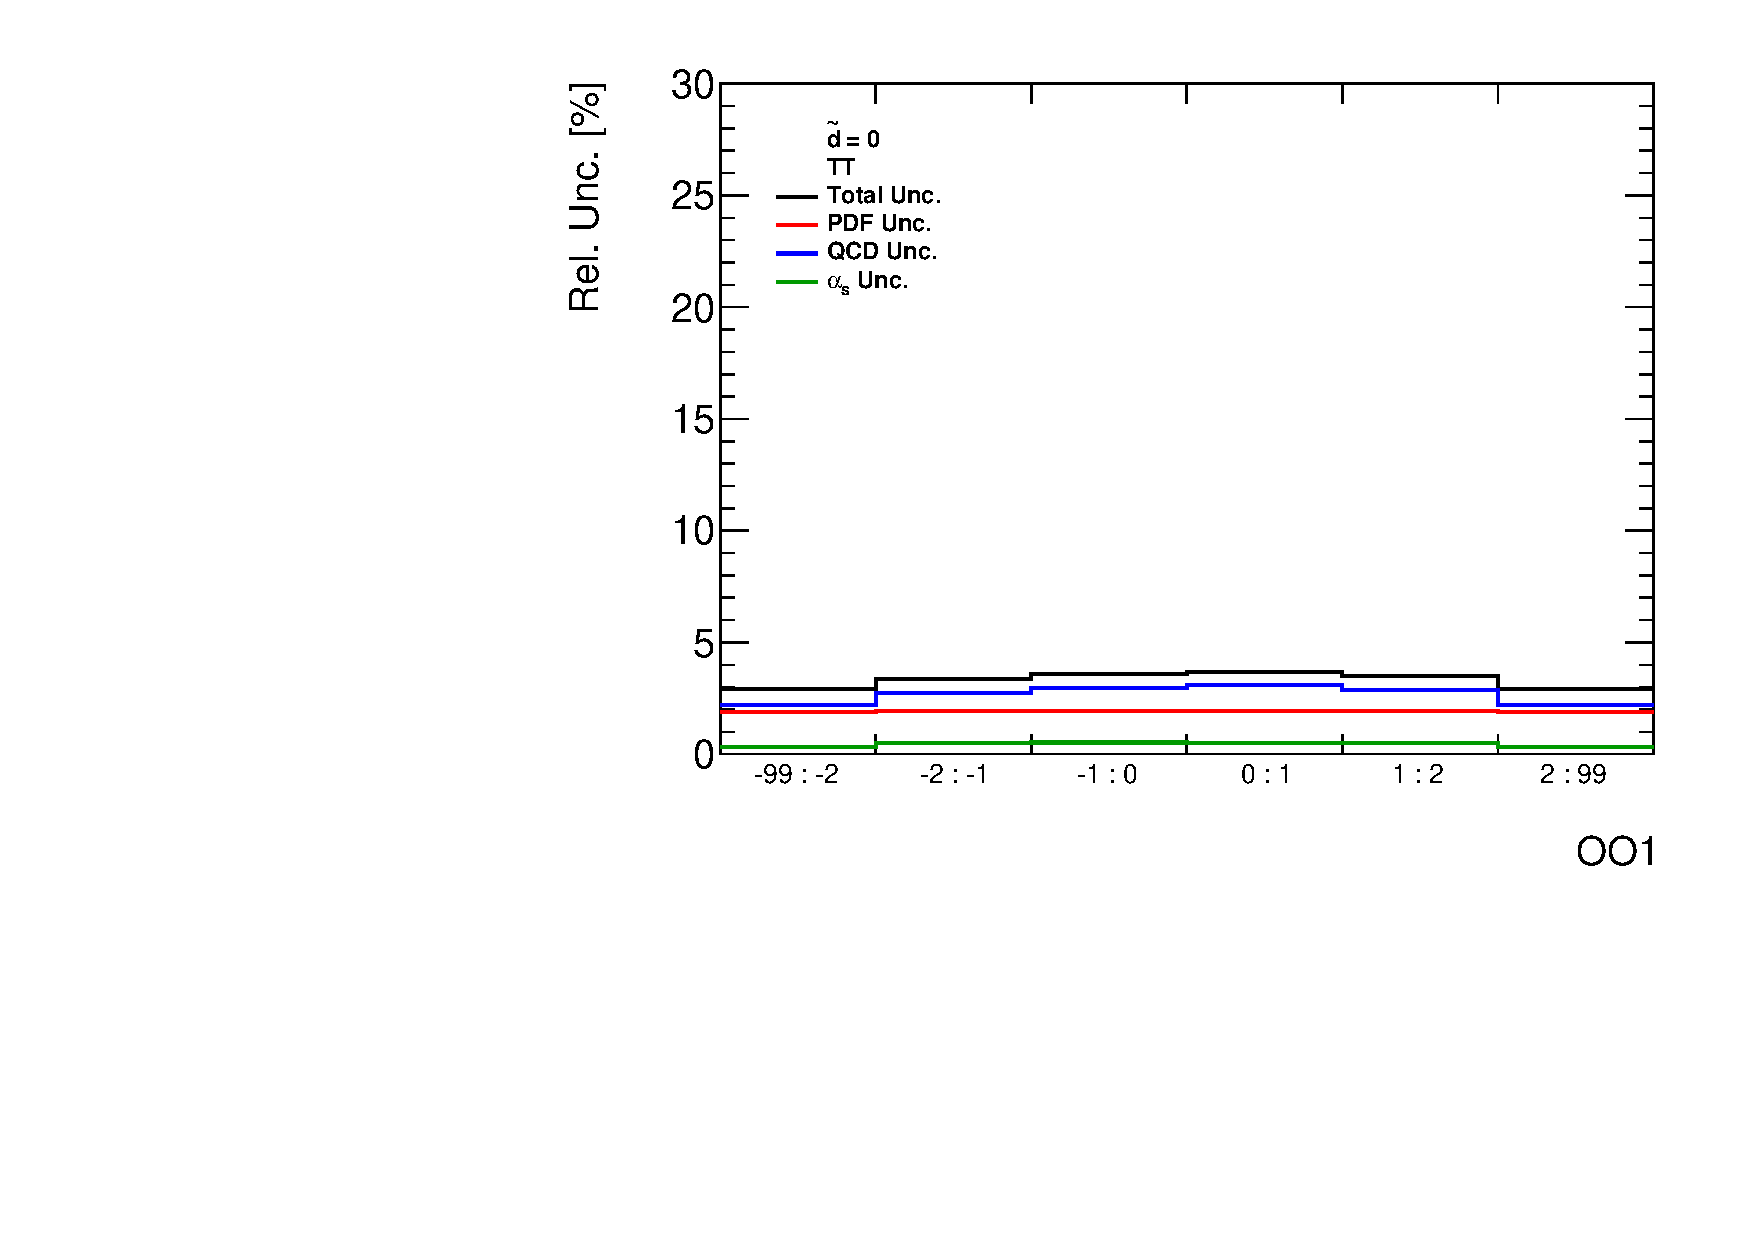
\includegraphics[width= 0.5\textwidth]{figure/TheorySyst/VBF_theoryUnc_TT_d_0.pdf} }
  \subfloat[TL ]{ 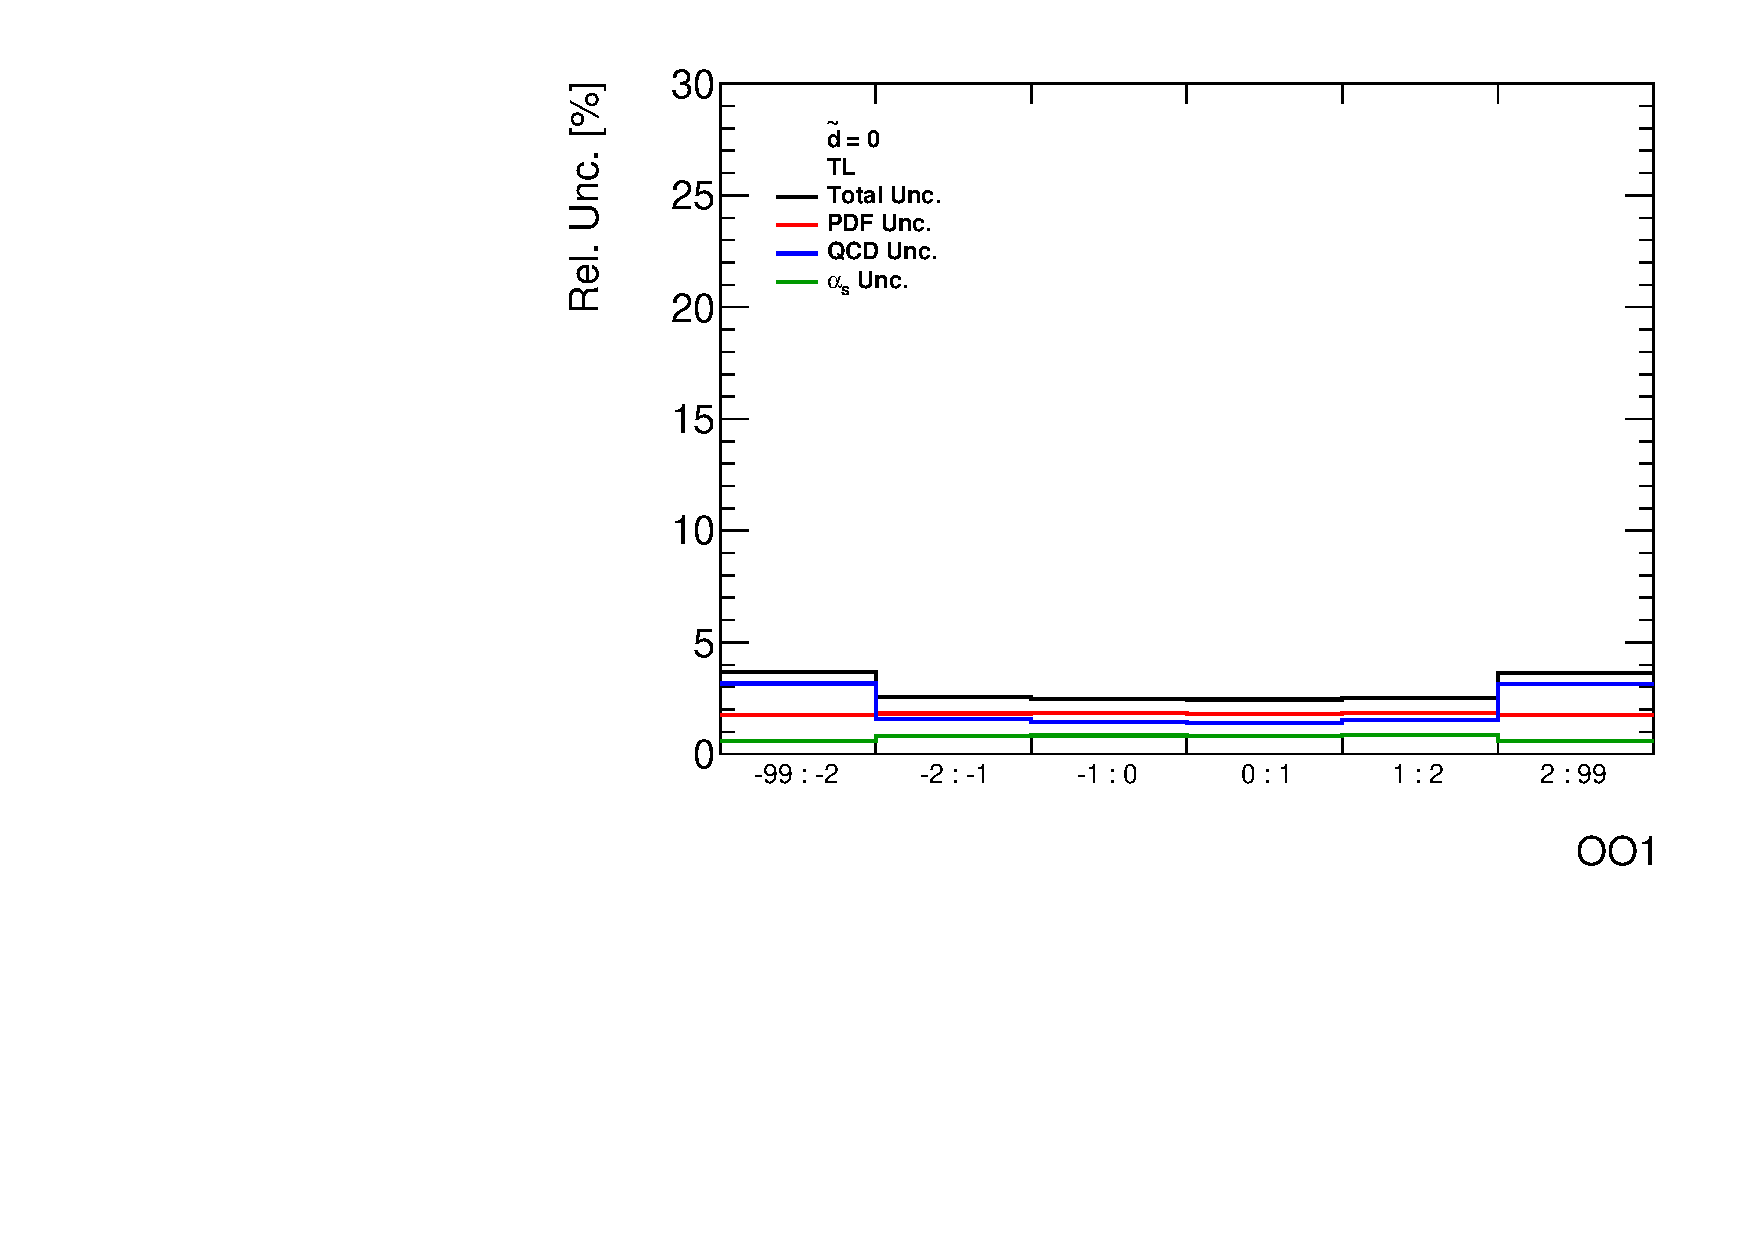
\includegraphics[width= 0.5\textwidth]{figure/TheorySyst/VBF_theoryUnc_TL_d_0.pdf} }\\
  \subfloat[LT ]{ 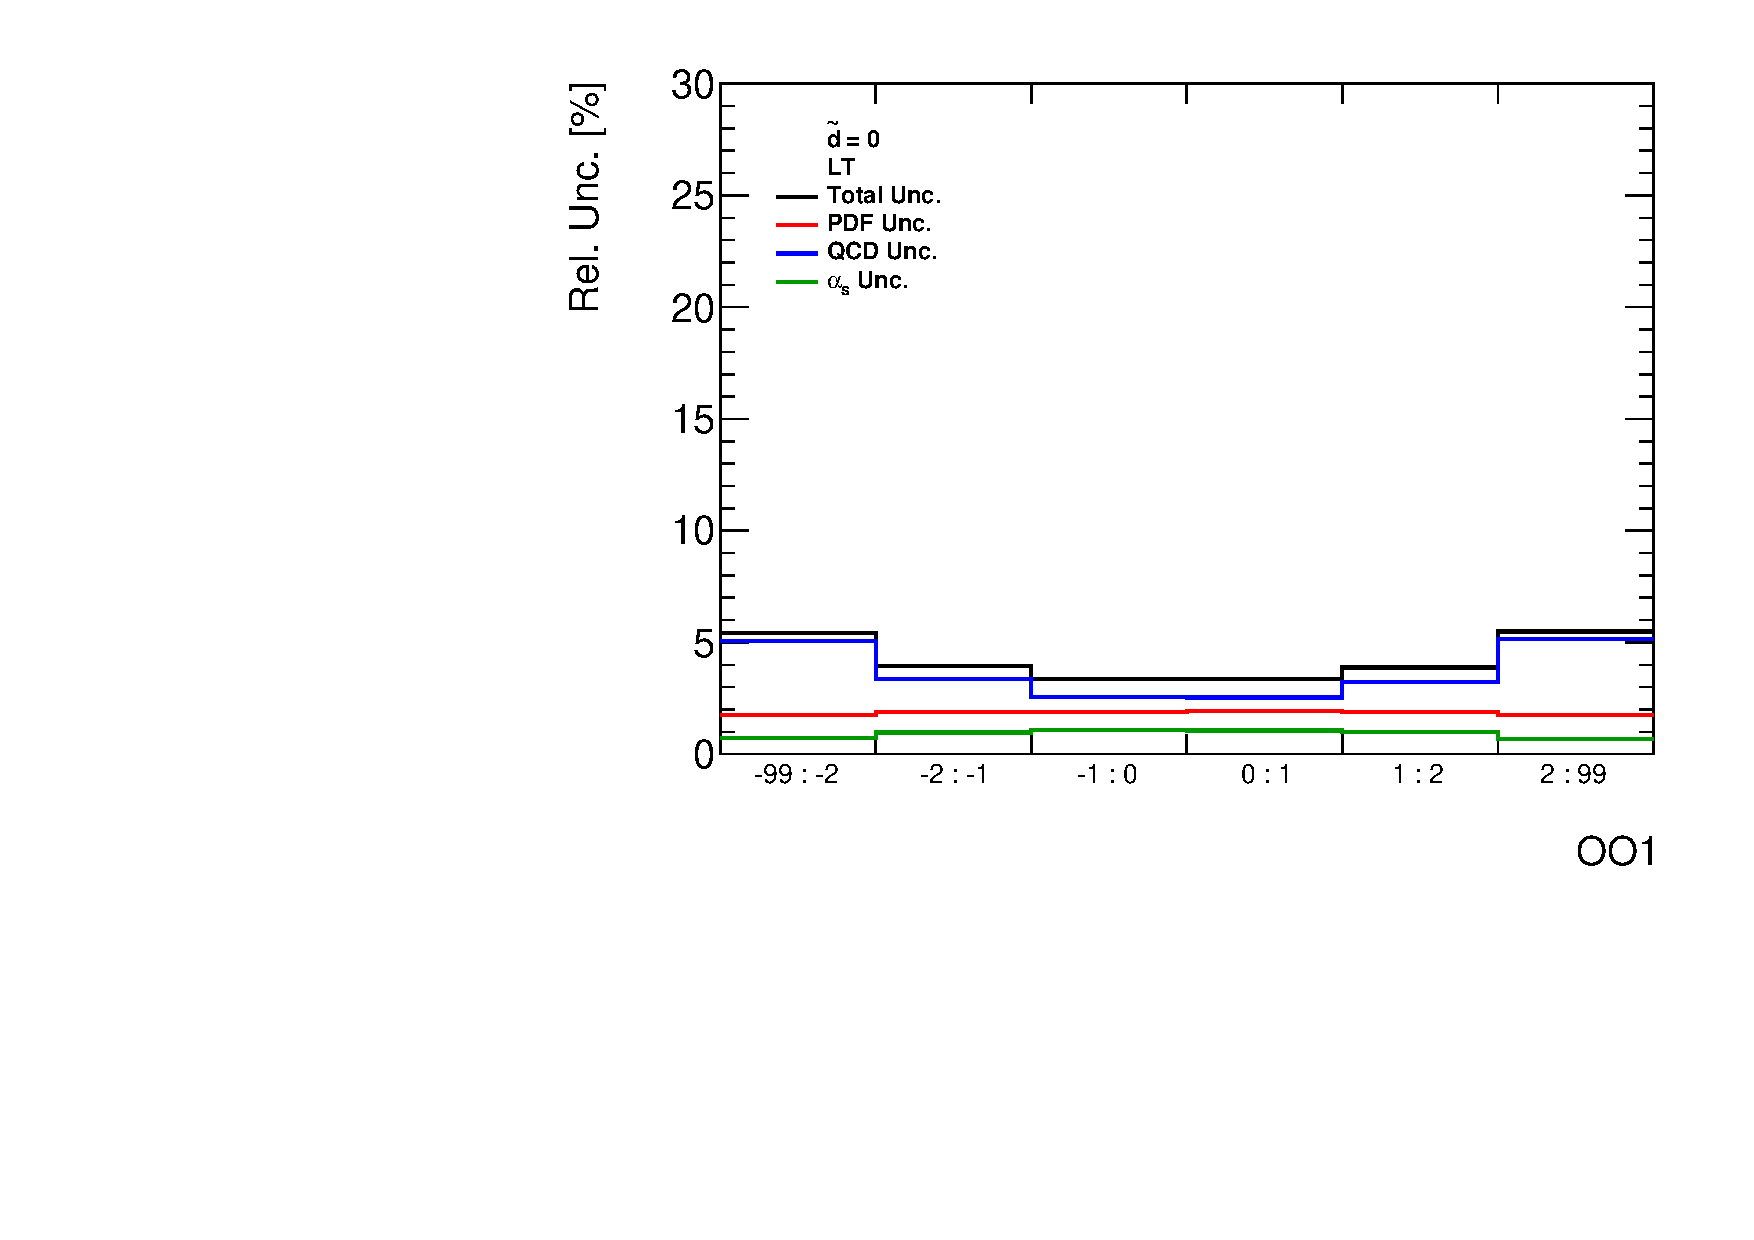
\includegraphics[width= 0.5\textwidth]{figure/TheorySyst/VBF_theoryUnc_LT_d_0.pdf} }
  \subfloat[LL ]{ 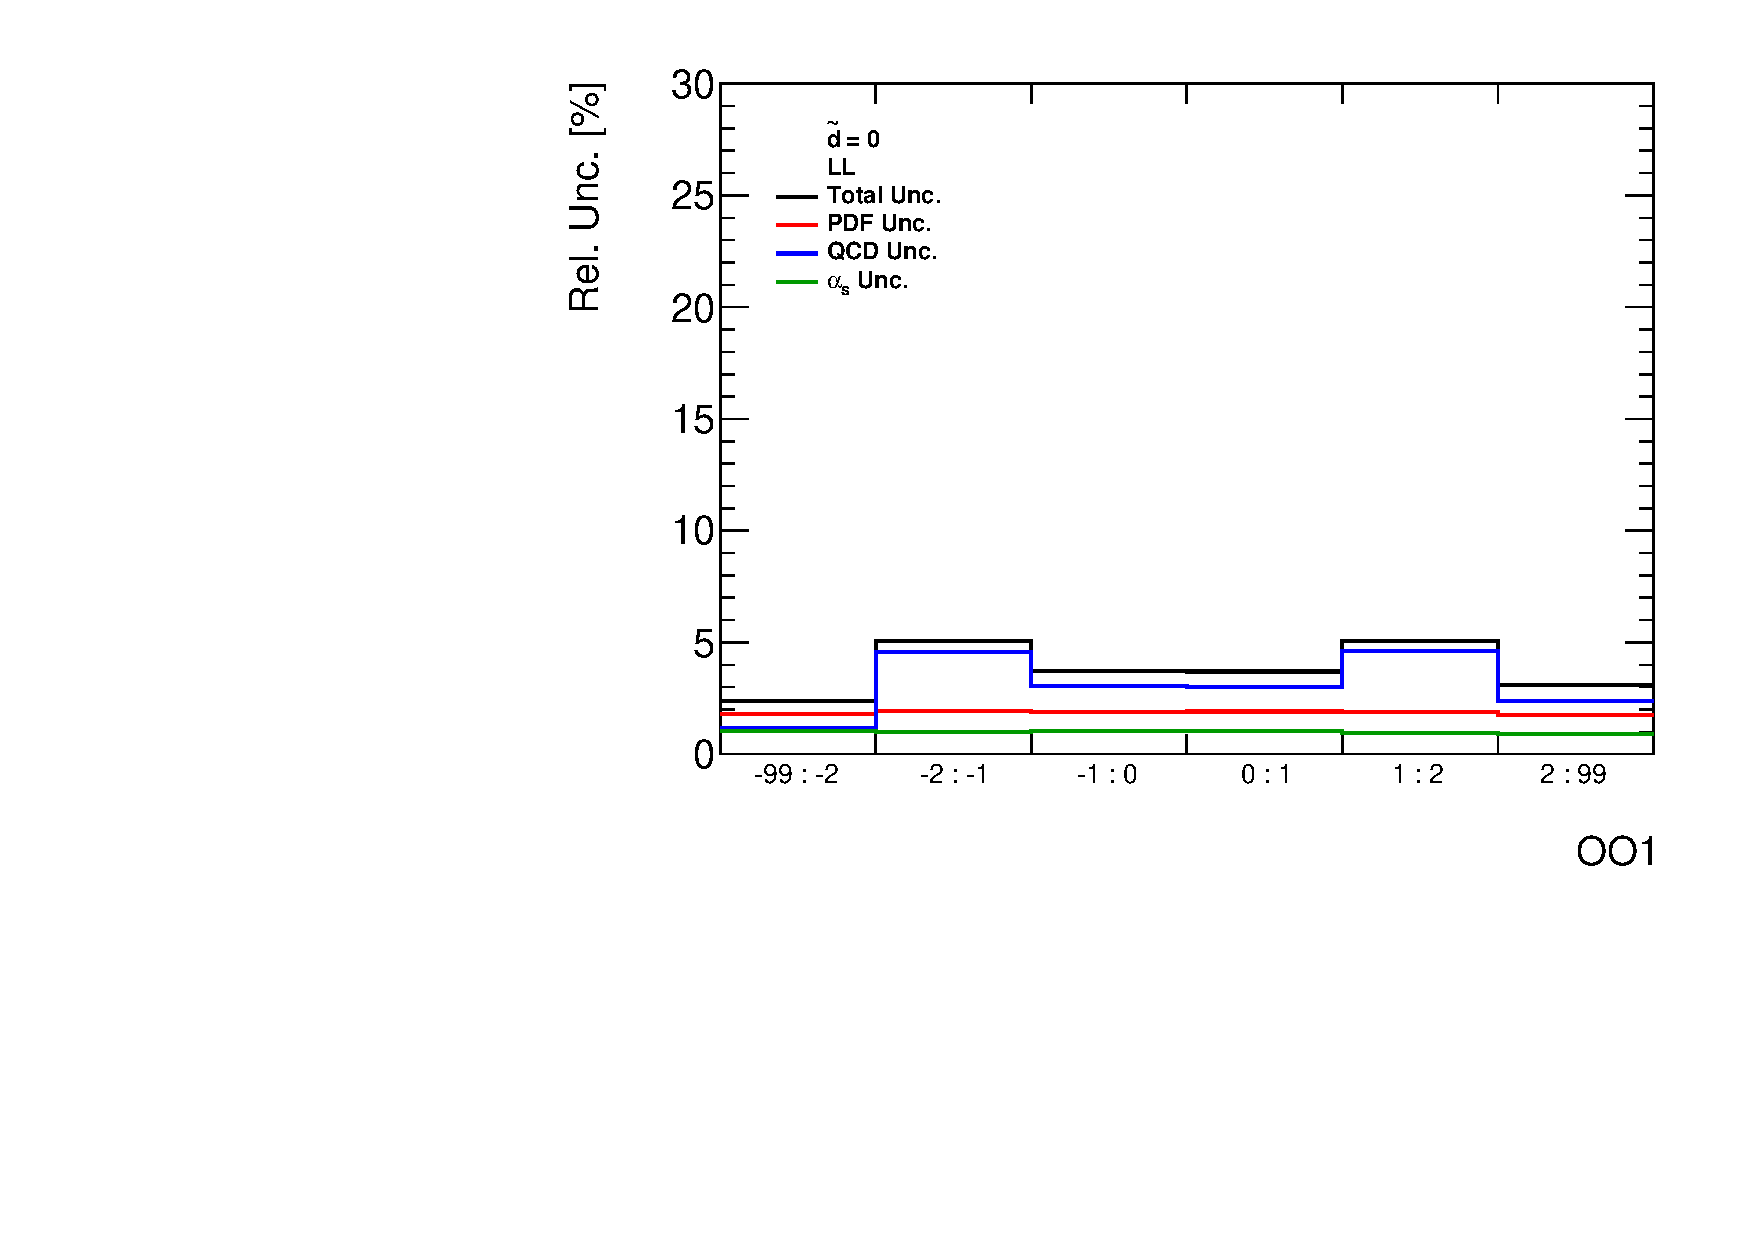
\includegraphics[width= 0.5\textwidth]{figure/TheorySyst/VBF_theoryUnc_LL_d_0.pdf} }
  \caption{Theory uncertainty in different OO bins for VBF process}
  \label{fig:theoryUnc_VBF}
\end{figure}




\subsection{Uncertainties from signal and background modeling}
\label{ssec:modeluncert}

\paragraph{} The Higgs peak described by double-side crystal ball function can be influence by several experimental effects. 
Photon energy scale uncertainties shift the position of signal peak by between $\pm0.2\%$ and $\pm0.4\%$, while the photon resolution uncertainties change the width of signal peak by between $\pm 6\%$ and $\pm 15\%$, following Ref ~\cite{ref:phscaleres}. 
Uncertainty due to knowledge of Higgs boson mass of 0.24GeV ~\cite{ref:mHerror} would also affect the signal peak position. 
These sources are considered independently into systematic uncertainties. 
\# \textcolor{red}{NUMBER NEED CHECK}
\todo{either add tables with full numbers here or in the signal section}
\paragraph{} The uncertainty due to the background choice is taken to be the spurious signal yield discussed in \Sect{\ref{ssec:spurious_signal}}, and assumed to be uncorrelated in each bins. 


\subsection{Experimental uncertainties}
\label{ssec:expuncert}

Experimental uncertainties could act both on the signal shape and expected category yields. Uncertainties on the shape are due to uncertainties on the photon energy scale and resolution, while uncertainties on the yield are due to object (photons and jets in this analysis) reconstruction and identification criteria.

Other yield systematics comprehend the spurious signal (1NP per category), the measured integrated luminosity (2\% systematic effect) the combined ATLAS-CMS Higgs mass uncertainty and the pileup
reweighting.

\subsubsection{signal shape uncertainties}
\label{sssec:shapeuncer}

The photon energy scale (PES) and the photon energy resolution (PER) variations act both on the signal shape and on the categories yields. Their effect is included in the fit to data as response functions on $\mu_{\mathrm{CB}}$ and $\sigma_{\mathrm{CB}}$, respectively. The other parameters of the Double Sided Crystal Ball function used to model the signal are not affected. These systematic variations are extracted for each analysis category and are treated as fully correlated among categories. The full coupling analysis is expected to be more sensitive to the PER than to the PES, since change in resolution affect our S/B ratio.



The uncertainties are computed from MC signal samples with all production processes merged according to the predicted SM fractions, using the following techniques:
\begin{itemize}
	\item for the \textbf{scale}, the ratio-of-mean technique is used: the means of $m_{\gamma\gamma}$ are computed for nominal and $\pm1\sigma$ varied distributions. Then, the systematic uncertainty applied to $\mu_{\mathrm{CB}}$ is evaluated as
	\begin{equation}
	\delta\mu_{\mathrm{CB}}^{\pm1\sigma}=\frac{\langle m_{\gamma\gamma}^{\pm1\sigma}\rangle}{\langle m_{\gamma\gamma}^{\mathrm{nom}}\rangle}-1
	\end{equation}
	Scale uncertainties are implemented in the fit to data with a \textcolor{red}{Gaussian constraint using the $\pm1\sigma$ variation, because of the high symmetry observed.} All the constraints are multiplied together and then applied to $\mu_{\mathrm{CB}}$ as a response function. The shift produced in the signal peak is usually below \textcolor{red}{0.3\%}, depending on the category, \textcolor{red}{which the high uncertainty usually represented by the L2 Gain systematic}. A couple of plots for the two first two 0 jet categories are reported in \textcolor{red}{Figure}
	\item for the resolution, the ratio of inter-quartile distribution is use: the inter-quartile is computed as $S=CDF^{-1}(75\%)-CDF^{-1}(25\%)$, where CDF is the cumulative distribution function of the $m_{\gamma\gamma}$ nominal and varied distributions. Then, the uncertainty is evaluated as
	\begin{equation}
	\delta\sigma_{\mathrm{CB}}^{\pm1\sigma}=\frac{S^{\pm1\sigma}}{S^{\mathrm{nom}}}-1
	\end{equation}
	Resolution \textbf{uncertainties} are implemented in the fit with an asymmetric constraint, to take into account differences in the $+1\sigma$ and $-1\sigma$ variations. All the resolution constraints are multiplied
together and then applied to $\sigma_{\mathrm{CB}}$ as a response function. The variations on the PER usually affect the signal resolutions by between \textcolor{red}{1\% and 8\%}. A couple of plots for the two first two 0 jet categories are reported in \textcolor{red}{Figure}
\end{itemize}

\textbf{Correlation mode}l Two models are provided by the calibration group: the first with 2 nuisance parameters (one for the scale and one for the resolution uncertainties), the latter with 80 systematics sources, 71 of which dedicated to scale uncertainties. As in the previous analysis, we will be able to constrain the 1NP model, so we have to go for the full one\textcolor{red}{: in particular, we use a full decorrelated model for the resolution (9 NPs) and a merged one for the scale (40 NPs, since we are not so sensitive to scale variations): the NPs related to the material in front of the calorimeter (MATCALO and MATCRYO), to the presampler (PS) and to S12, which are divided in many $\eta$ bins, are sum together in two contributions each, one bin for the barrel and one for the endcap region.}

\subsubsection{signal yield uncertainties}
\label{sssec:yielduncer}

Yield uncertainties act on the yield of a given reconstructed category and truth bin, letting events migrate among them or changing the efficiency of the diphoton selection.

85 experimental systematic sources are taken into account: the main experimental systematics are jet reconstruction uncertainties, especially jet flavour composition, flavour response, modelling, topology, jet energy resolution and photon uncertainties on isolation and identification efficiency. Other important sources come from pileup modelling in simulation and spurious signal, see \textcolor{red}{Section 8.2.3}. Uncertainties on the measured luminosity and on the efficiency of diphoton trigger are computed and taken into account. Concerning the impact of PER and PES on the category yield, since this is usually smaller than other systematic sources, we have decided to use the 1NP schemes here. Concerning instead the PRW systematic this is computed applying the standard ATLAS correction factors (up/down variation of 1/0.94 and 1/1.12). These values are computed as the relative difference between $\pm1\sigma$ varied yields and the nominal one using signal MC samples:

\begin{equation}
\delta n_{\mathrm{c}}^{\pm1\sigma}=\frac{ n_{\mathrm{c}}^{\pm1\sigma}}{n_{\mathrm{c}}^{\mathrm{nom}}}-1
\end{equation}
Systematic uncertainties are computed for each reconstructed category $c$. Each source of systematic uncertainty is treated as fully correlated among truth bin and categories. \textcolor{red}{The systematic sources which have only $+1\sigma$ variation (like $E_{T}^{\mathrm{miss}}$ soft track term resolution) are implemented in the fit with log-normal constraints; all the others have instead} an asymmetric constraint since up and down variations could have different values. A couple of plot showing the impact of the experimental systematic sources on a \textcolor{red}{ggH 1J category and on a VBF one are shown in Figure}

\textcolor{red}{\textbf{Pruning} Due to these large amount of systematics variations we need to insert in the workspace, a pruning criterium has been applied in order to remove response functions with a very low impact or an incorrect evaluation due to limited MC statistic. A systematic variation for a certain category-process couple is pruned if
\begin{itemize}
	\item up or down variation is null: $\delta n_{\mathrm{c}}^{+1\sigma}=0$ or $\delta n_{\mathrm{c}}^{-1\sigma}=0$;
	\item up and down variations show a large difference: $|\delta n_{\mathrm{c}}^{+1\sigma}/\delta n_{\mathrm{c}}^{-1\sigma}|>10$ or $|\delta n_{\mathrm{c}}^{-1\sigma}/\delta n_{\mathrm{c}}^{+1\sigma}|>10$(so large differences are only expected in case of lacking of MC statistics);
	\item variations are both small: $\delta n_{\mathrm{c}}^{+1\sigma}<0.3\%$ and $\delta n_{\mathrm{c}}^{-1\sigma}<0.3\%$
\end{itemize}
Moreover the sources with same sign variations are modified in order to have a positive $\delta n_{\mathrm{c}}^{+1\sigma}$ and a negative $\delta n_{\mathrm{c}}^{-1\sigma}$}

\textcolor{red}{To estimate the statistical uncertainty on the effect of a given systematic variation on the signal yield, a bootstrap technique has been implemented to obtain a statistical error on their values. Three thousands pseudo-yields are generated for nominal, up and down variations of any systematic source, using correlated Poissonian weights (in fact, a resampling technique); then, the bootstrapped $\delta n_{\mathrm{c}}$ is calculated for each of them and the statistical error is estimated as the standard deviation of distribution($\sigma_{\delta n_{\mathrm{c}}}$).}

\textcolor{red}{old-new division line}


\todo{too concise, please detail and split jet, photons sources and write one line how these variations are estimated, add OO plots showing the sys. variations (i have those plots)}
\paragraph{} With data taken during 2015-2018, the uncertainty from integrate luminosity is 2.0\%. Other sources of experimental uncertainty affecting the expected signal yields include: the efficiency of diphoton trigger, the photon identification and isolation efficiencies, the photon energy scale and resolution, the modelling of pile-up in the simulation, the jet energy scale and resolution, the efficiency of the jet vertex tagger. Among them the dominant one is jet flavor composition \texttt{ATLAS\_JET\_Flavor\_Composition} which contributes 5.5\%. \\

The considered systematic uncertainty terms are shown in Figure ~\ref{fig:syst_ranking}. 

\todo{the ranking plot doesn't belong in this section, should be in the next}
\begin{figure}[h]
  \centering
  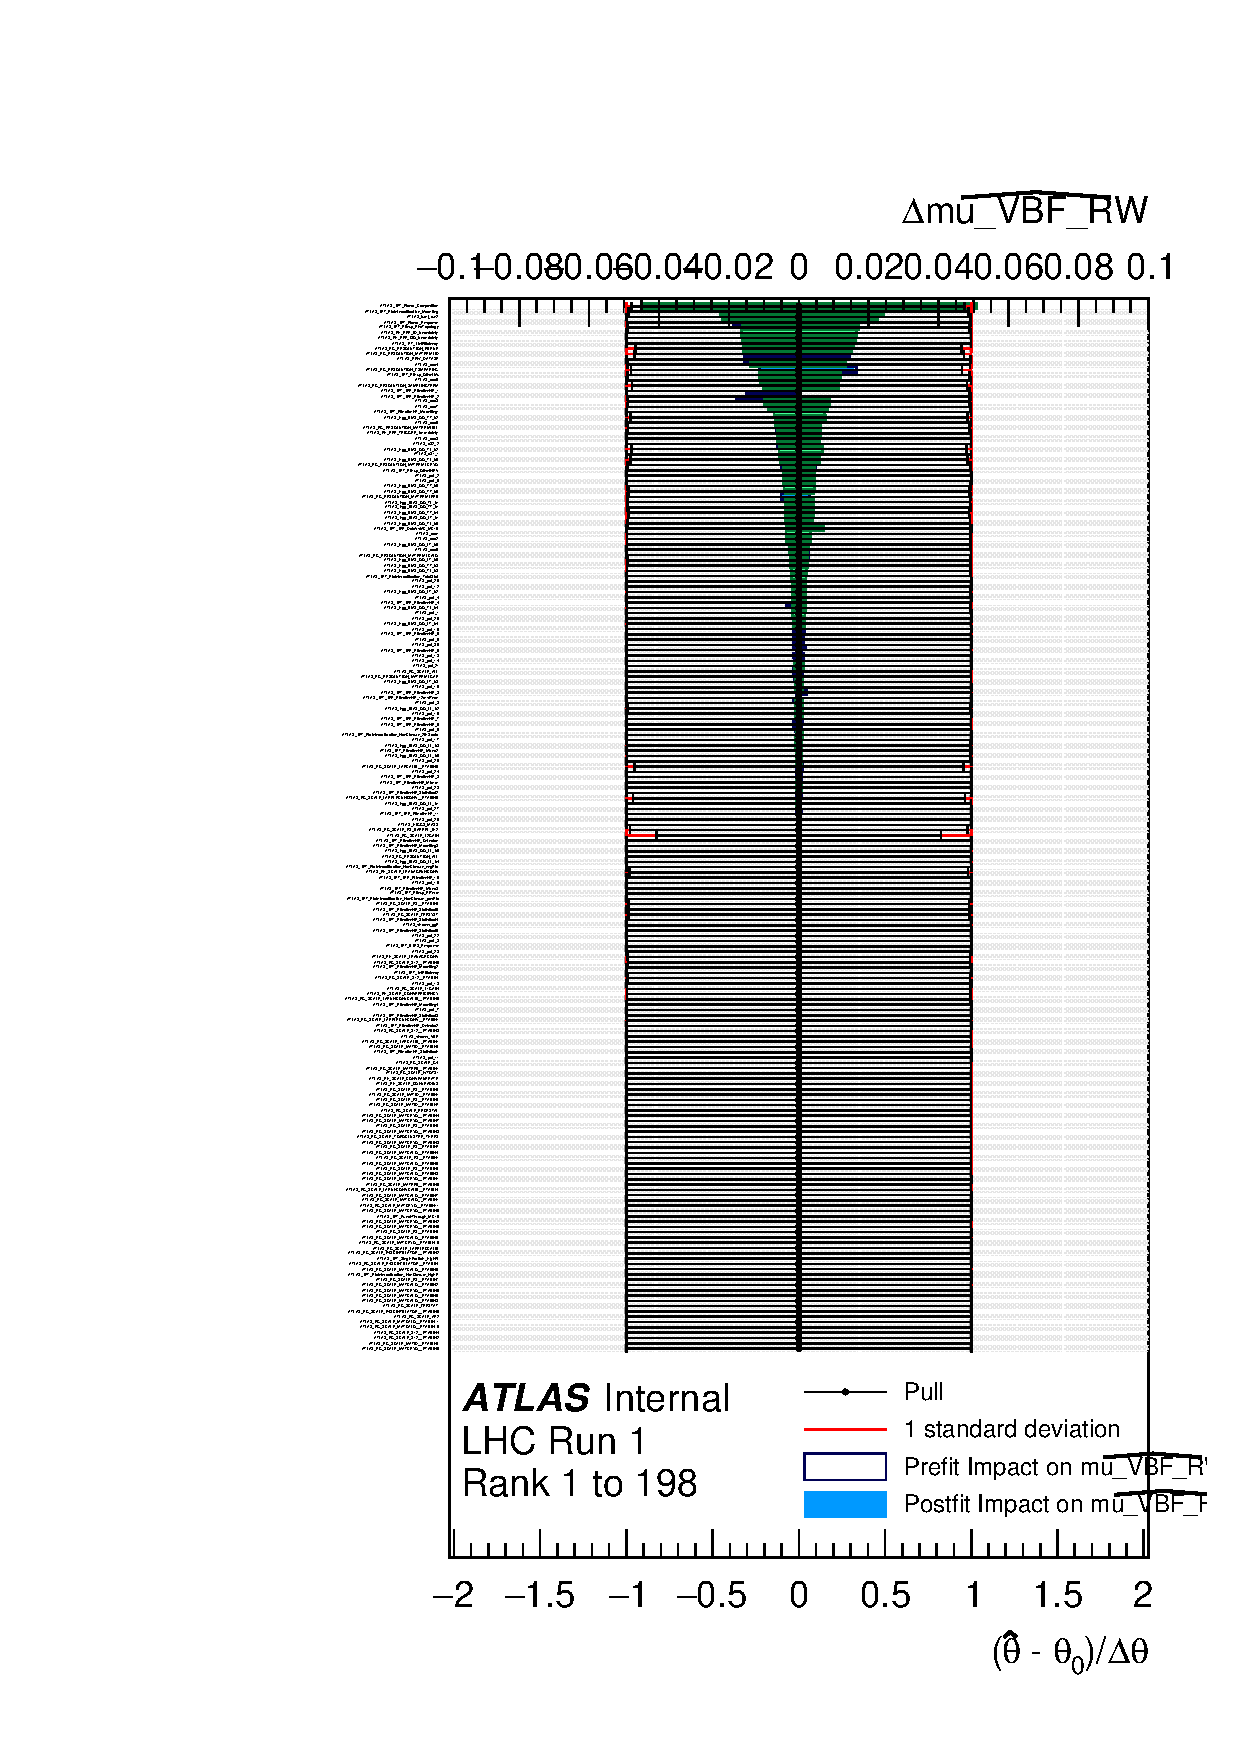
\includegraphics[width=.9\textwidth]{figure/ranking.pdf}
  \caption{Ranking plot for all systematic uncertainty terms. }
  \label{fig:syst_ranking}
\end{figure}


